\documentclass[a4paper,12pt]{article} 
\usepackage[T2A]{fontenc}			
\usepackage[utf8]{inputenc}			
\usepackage[english,russian]{babel}	
\usepackage{amsmath,amsfonts,amssymb,amsthm,mathtools} 
\usepackage[colorlinks, linkcolor = blue]{hyperref}
\usepackage{upgreek}
\usepackage[left=2cm,right=2cm,top=2cm,bottom=3cm,bindingoffset=0cm]{geometry}
\usepackage{multirow}
\usepackage{graphicx}
\usepackage{xcolor}
\usepackage{multirow}
\usepackage{pgfplots}
\usepackage{pgfplotstable}
\pgfplotsset{compat=1.9}

\pgfplotstableset{ %
        create on use/SquareLight/.style={
                create col/expr={\thisrow{Dark}}}
}

\author{Шелихов Дмитрий\\Группа Б01-305}

\title{\textbf{Работа 3.6.1\\Cпектральный анализ электрических сигналов}} 
\date{\today}

\begin{document} 

\maketitle

\textbf{Цель работы:} изучить спектральный состав периодических электрических сигналов.
\par
\textbf{В работе используются:} анализатор спектра (аналоговый или цифровой), генератор прямоугольных импульсов и сигналов специальной формы, осциллограф.\\
\noindent\textbf{Теоретическая справка}

Периодическая функция может быть представлена в виде бесконечного ряда гармонических функций - ряда Фурье:

$$ f(t) = \sum\limits_{n=-\infty}^{\infty} c_ne^{in\omega_0t}  $$

$$\omega_0 = 2\pi/T \text{,где T - период функции f(t). Коэффициенты {$c_n$} могут быть найдены по формуле: }$$
$$ c_n = \frac{1}{T}\int_0^Tf(t)e^{-inw_0t}dt. $$

Простейший спектральный анализатор - высокодобротный колебательный контур с подстраиваемой ёмкостью или индуктивностью.

\center{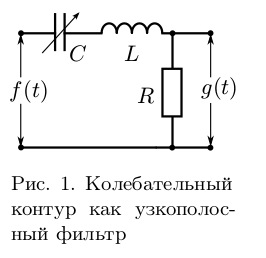
\includegraphics[width=.4\textwidth]{1.png}}

Такой контур усиливает гармоники входного сигнала f(t), частота которых близка к резонансной $\nu_0$ = $\frac{1}{2\pi\sqrt{LC}}$, и практически не реагирует на частоты, далёкие от $\nu_0$. Таким образом, с точки зрения преобразования сигналов, такой контур является является узкополосным фильтром с шириной полосы пропускания порядка $\Delta\nu \approx \nu_0/Q$, где Q = $\frac{1}{R}\sqrt{\frac{L}{C}}$ >> 1 - его добротность.  

При этом амплитуда колебаний в контуре пропорциональна амплитуде |c($\nu_0$)| гармоники в спектре функции f(t), частота которой совпадает с $\nu_0$. Таким образом, меняя резонансную частоту контура, можно просканировать весь спектр входного сигнала. \\

\noindent \textbf{Экспериментальная установка}
	Рассмотрим следующую схему: 	
Исследуемый сигнал f(t) и синусоидальный сигнал от вспомогательного генератора, называемого в таких системах \textbf{гетеродином}, подаются на вход \textbf{смесителя}. Смеситель преобразует колебания с частотами $\nu_1$ и $\nu_2$ в колебания на комбинированных частотах: $\nu1 + \nu2$ и $\nu1 - \nu2$. Сигнал смесителя поступает на фильтр, настроенный на фиксированную резонансную частоту $\nu_0$. То есть, если f(t) содержит гармонику $\nu = \nu_{гет} - \nu_0$, она будет усилена, а отклик будет пропорционален её амплитуде.

\center{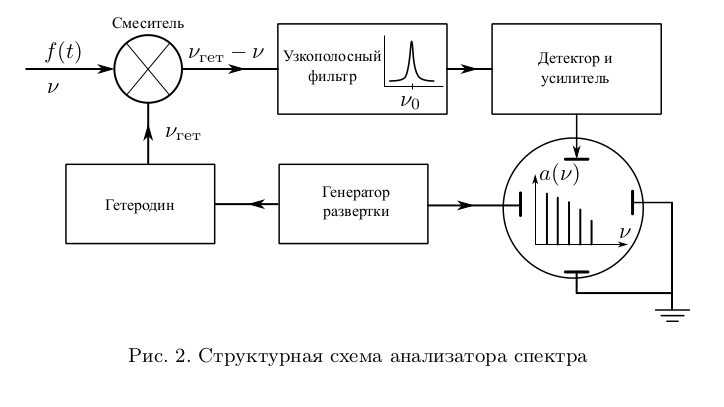
\includegraphics[width = .8\textwidth]{2.png}}

На экране анализатора возникает график, изображающий зависимость амплитуды гармоник исходного сигнала от частоты, т.е. его спектр.\\

\textbf{Ход работы}\\

\textbf{А. Исследование спектра периодической последовательности прямоугольных импульсов}\\

Исследуем зависимость ширины спектра $\Delta\nu$ периодической последовательности прямоугольных импульсов от длительности отдельного импульса $\tau$. 

\noindent 1) Ознакомимся с устройством приборов: генератор прямоугольных импульсов, осциллограф, анализатор спектра и подготовим их к работе, следуя техническим описаниям. 

\center{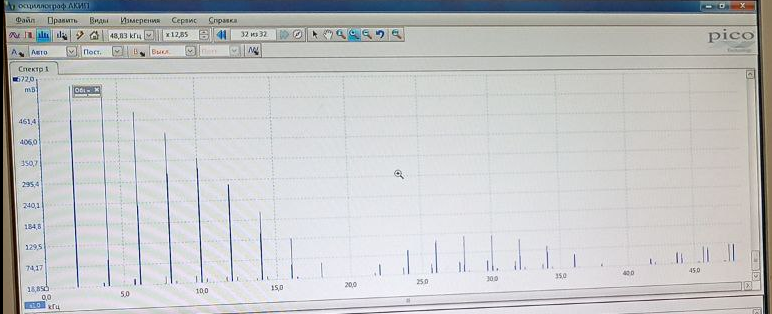
\includegraphics[width=.8\textwidth]{3.png}}

\noindent 2) Подключим генератор прямоугольных импульсов через разветвитель к осциллографу и анализатору спектра.

\noindent 3) На генераторе зададим частоту повторения импульсов $\nu_{\text{повт}}$ = 1кГц (период T = 1мс), длительность импульса $\tau$ = 50 мкс. Получим устойчивую картину сигнала на осциллографе. 

\noindent 4) Предварительно оценим характерную ширину спектра из соотношения неопределённостей $\Delta\nu \approx 1/\tau$ = 20 кГц. 

\noindent 5) Получим спектр сигнала на анализаторе спектра. Предварительно подберём начало отсчёта и диапазон измерения по частоте, так чтобы на экране помещалась большая часть спектра.

\noindent 6) Изменяя параметры сигнала ($\nu_{\text{повт}}$, $\tau$), пронаблюдаем как изменяется его спектр.

\begin{figure}[h]
\center{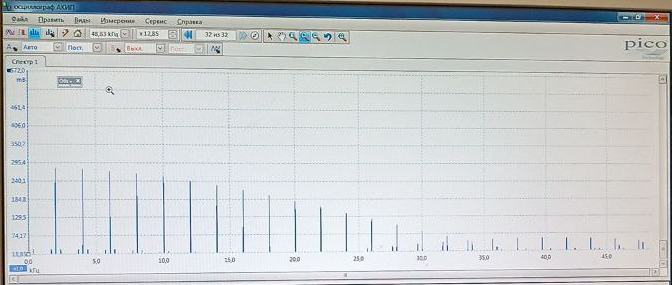
\includegraphics[width=.6\textwidth]{4.png}}
\caption{$\nu_{\text{повт}}$ = 1кГц, $\tau$ = 50мкс}
a) Картинка для сравнения
\end{figure}

\begin{figure}[h]
\center{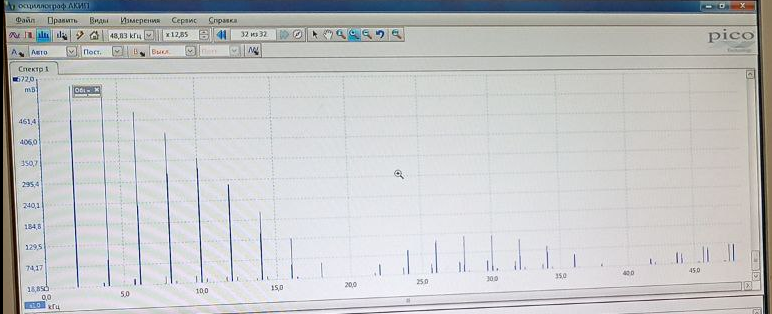
\includegraphics[width=.6\textwidth]{5.png}}
\caption{$\nu_{\text{повт}}$ = 2кГц, $\tau$ = 50мкс}
б) При увеличении $\nu_{\text{повт}}$ амплитуды гармоник увеличиваются, ширина спектра не меняется.
\end{figure}

\begin{figure}[h]
\center{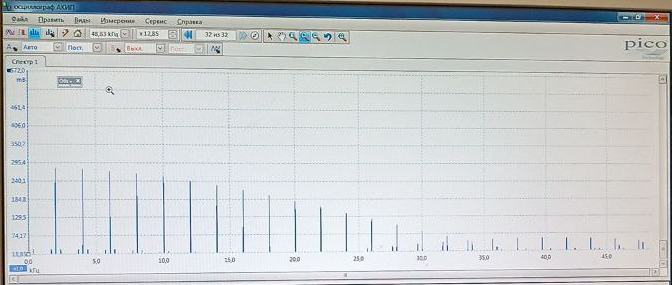
\includegraphics[width=.6\textwidth]{6.png}}
\caption{$\nu_{\text{повт}}$ = 2кГц, $\tau$ = 25мкс}
в) При уменьшении $\tau$ амплитуды уменьшаются, ширина спектра увеличивается.
\end{figure}

\begin{figure}[h]
\center{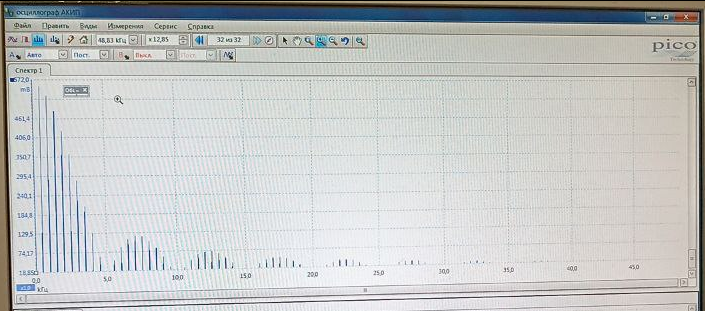
\includegraphics[width=.6\textwidth]{7.png}}
\caption{$\nu_{\text{повт}}$ = 0,5кГц, $\tau$ = 200мкс}
г) Амплитуды возросли, ширина спектра уменьшилась. (в результате суперпозиции пунктов б и в) 
\end{figure}

Масштаб частот по оси X на всех изображениях один и тот же.

\noindent 7) Проведём измерения зависимости ширины спектра от длительности импульса $\Delta\nu$($\tau$) при изменении $\tau$ от 25 до 200 мкс при $\nu_{\text{повт}}$ = 1 кГц. Ширину определяем по положению первой гармоники с нулевой амплитудой.

\begin{center}
\begin{tabular}{|c|c|c|}
	\hline
	$\tau$, мкс & $\Delta\nu$, кГц & $\nu_{\text{повт}}$, кГц \\
	\hline
	30 & 27,8 $\pm$ 1.4  & \multirow{6}{*}{1}\\
	\cline{1-2} 45 & 19,9 $\pm$ 1.0 & \\
	\cline{1-2} 67,5 & 13,8 $\pm$ 0.7 & \\
	\cline{1-2} 100 & 10.0 $\pm$ 0.5 & \\
	\cline{1-2} 140 & 6,0 $\pm$ 0.3 & \\
	\cline{1-2} 200 & 5,0 $\pm$ 0.1 & \\
	\hline
\end{tabular}
\end{center}

\noindent 8) Построим график зависимости ширины спектра от обратного времени импульса $\Delta\nu(1/\tau)$.

\pgfplotstableread{
x			y 		y-max 	y-min
5			5.0		0.1		0.1
7.14286		6.0		0.3		0.3
10			10.0	0.5		0.5
14.81481	13.8	0.7		0.7
22.22222	19.9	1.0		1.0
33.33333	27.8	1.4		1.4
}{\mytable}

\begin{tikzpicture}
\begin{axis} [
	title = $\Delta\nu(1/\tau)$,
	xlabel = {1/$\tau$, кГц},
	ylabel = {$\Delta\nu$, кГц},
	minor tick num = 2,
	grid = major
]

\addplot +[mark options = {scale = 0.1,}]
	plot [error bars/.cd, y dir=both, y explicit]
	table [y error plus=y-max, y error minus=y-min] {\mytable};

\addplot +[mark options = {scale = 0,}]
	table[row sep=\\,				%аппроксимация
   y={create col/linear regression={y=Y}}]
    {
   		X Y\\  
		33.33333  27.8 \\    
		22.22222  19.9\\   
		14.81481  13.8\\   
		10   10.0\\  
		7.14286   6.0\\    
		5   5.0\\     
    };
	\addlegendentry{
        k$\approx \pgfmathprintnumber{\pgfplotstableregressiona}$} 
\end{axis}
\end{tikzpicture}

Получили k $\approx$ 0.82 $\pm$ 0.05. По соотношению неопределённостей $k\approx\Delta\nu\cdot\tau\approx1$. Таким образом соотношение соблюдается, поскольку получена величина по порядку совпадающая с единицей.

\noindent 9) Для сигнала из первого изображения ($\nu_{\text{повт}}$ = 1кГц, $\tau$ = 50мкс) рассчитаем теоретические значения амплитуд спектральных компонент по формуле:

$$ {|c_n|}^{теор} = \frac{|sin\frac{\pi n\tau}{T}|}{\pi n} $$

\begin{center}
\begin{tabular}{|c|c|c|c|c|c|c|c|c|}
	\hline
	n гармоники & 1 & 2 & 3 & 4 & 5 & 6 & 7 & 8 \\
	\hline
	$\nu_n^{\text{эксп}}$, кГц & 1,014 & 2,031 & 3,007 & 4,024 & 5,041 & 6,017 & 6,994 & 8,011 \\
	\hline
	$\nu_n^{\text{теор}}$, кГц & 1 & 2 & 3 & 4 & 5 & 6 & 7 & 8 \\
	\hline
	$|c_n^{\text{эксп}}|$, мВ & 279,1 $\pm$ 0,1 & 275,8 $\pm$ 0,1 & 270,9 $\pm$ 0,1 & 262,7 $\pm$ 0,1 & 252,9 $\pm$ 0,1 & 241,4 $\pm$ 0,1 & 226,7 $\pm$ 0,1 & 212,0 $\pm$ 0,1 \\
	\hline
	${|c_n/c_1|}^{\text{эксп}}$ & 1 & 0,988 $\pm$ 0,001 & 0,967 $\pm$ 0,001 & 0,939 $\pm$ 0,001 & 0,904 $\pm$ 0,001 & 0,862 $\pm$ 0,001 & 0,814 $\pm$ 0,001 & 0,760 $\pm$ 0,001 \\
	\hline
	${|{c_n/c_1}|}^{\text{теор}}$ & 1 & 0,988 & 0,971 & 0,941 & 0,906 & 0,865 & 0,812 & 0,760 \\
	\hline
\end{tabular}
\end{center}

Сравним измеренные значения с теоретическими, изобразив их на одном графике.

\pgfplotstableread{
x	y 		y-max 	y-min
1	1	0.0	0.0
2	0.988	0.001	0.001
3	0.967 0.001 	0.001
4	0.939	0.001 	0.001
5	0.904	0.001 	0.001
6	0.862	0.001	0.001
7	0.814	0.001	0.001
8	0.760	0.001	0.001
}{\mytable}

\begin{tikzpicture}
\begin{axis} [
	title = $|c_n/c_1|$(n),
	xlabel = {n},
	ylabel = {$|c_n/c_1|$},
	minor tick num = 2,
	grid = major
]

\addplot +[mark options = {scale = 0.1,}]
	plot [error bars/.cd, y dir=both, y explicit]
	table [y error plus=y-max, y error minus=y-min] {\mytable};

\pgfplotstableread{
x   y       y-max   y-min
 1   1   0.0 0.0
 2   0.988   0.0   0.0
 3   0.971 0.0     0.0
 4   0.941   0.0   0.0
 5   0.906   0.0   0.0
6   0.865   0.0   0.0
7   0.812   0.0   0.0
8   0.760   0.0   0.0
}{\mytable}

\addplot +[mark options = {scale = 0.1,}]
     plot [error bars/.cd, y dir=both, y explicit]
     table [y error plus=y-max, y error minus=y-min] {\mytable};


\end{axis}
\end{tikzpicture}

\textbf{Б. Исследование спектра периодической последовательности цугов гармонических колебаний}

Исследуем зависимость расстояния между ближайшими спектральными компонентами от частоты повторения цугов.

\noindent 10) По техническому описанию к работе соберем схему, используемую для генерации последовательности синусоидальных цугов.

\noindent 11) Установим несущую частоту $\nu_0$ = 25кГц и получим на экране осциллографа устойчивую картину цугов.

\noindent 12) Получим спектр сигнала. Пронаблюдаем, как изменяется вид спектра:

Число N отвечает за число волн спектра, которое равно 2N-1.

 \begin{figure}
 \center{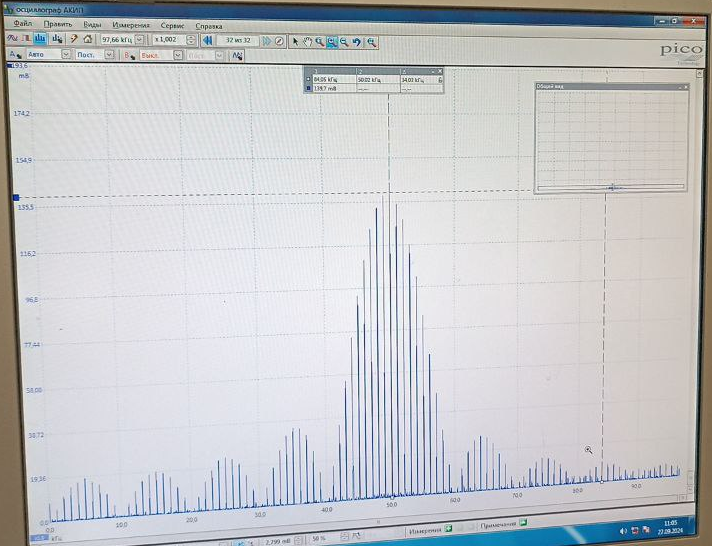
\includegraphics[width=.4\textwidth]{8.png}}
 \caption{$\nu_0$ = 50кГц, T = 1мс, N = 5}
 a) Картинка для сравнения
 \end{figure}


 
 \begin{figure}
 \center{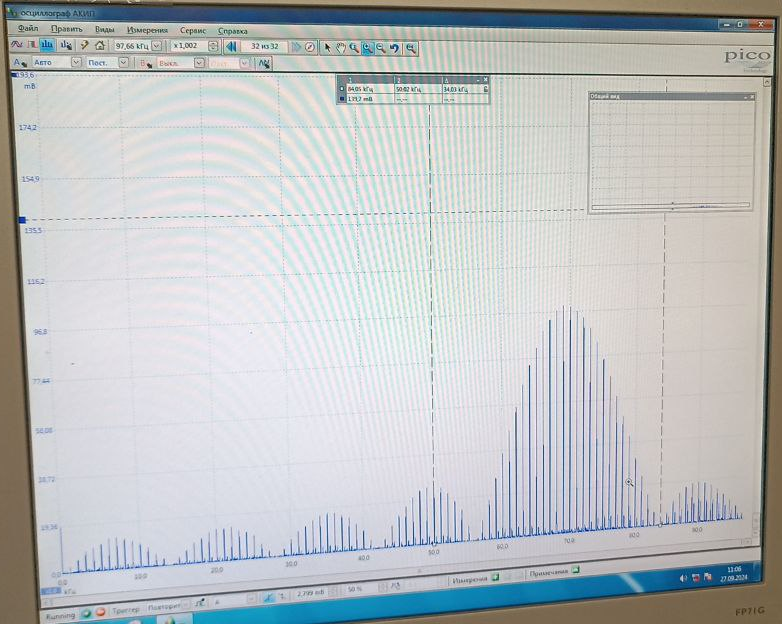
\includegraphics[width=.4\textwidth]{9.png}}
 \caption{$\nu_0$ = 70кГц, T = 1мс, N = 5}
 б) При увеличении $\nu_0$ амплитуды гармоник уменьшаются, ширина спектра увеличивается.
 \end{figure}
 


 \begin{figure}
 \center{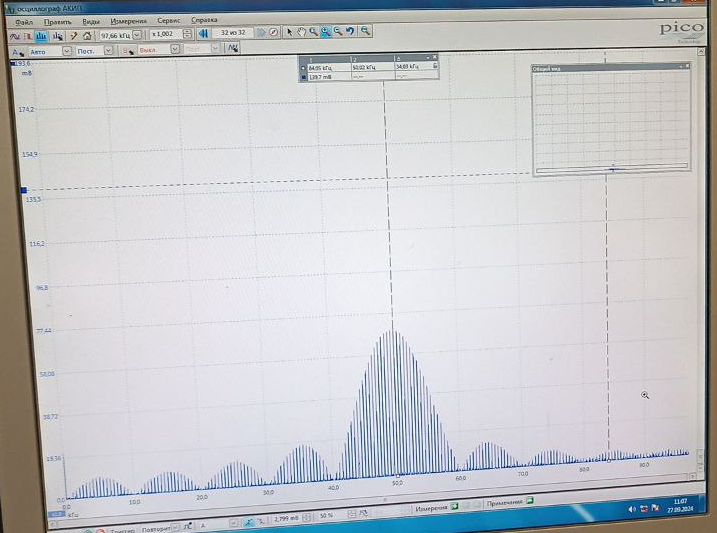
\includegraphics[width=.4\textwidth]{10.png}}
 \caption{$\nu_0$ = 50кГц, T = 2мс, N = 5}
 в) При увеличении T амплитуды уменьшаются, ширина спектра не меняется.
 \end{figure}


 
 \begin{figure}
 \center{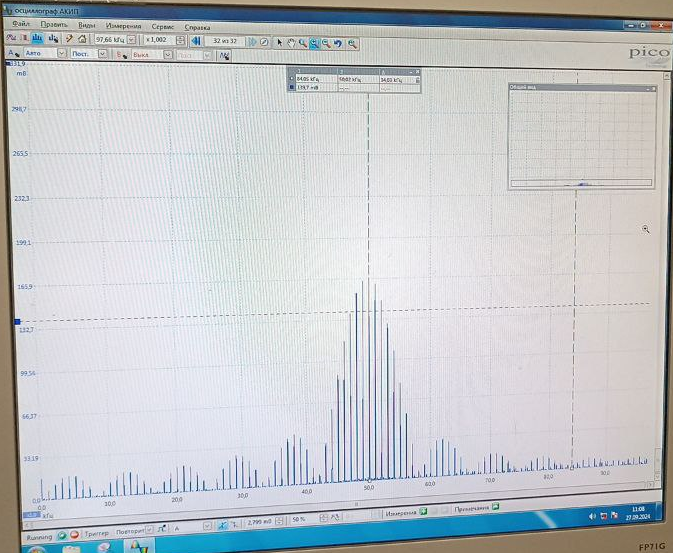
\includegraphics[width=.4\textwidth]{11.png}}
 \caption{$\nu_0$ = 50кГц, T = 1мс, N = 6}
 г) При увеличении N амплитуда растёт, ширина спектра уменьшается.
 \end{figure}
 


 Масштаб частот по оси X на всех изображениях один и тот же.

\center{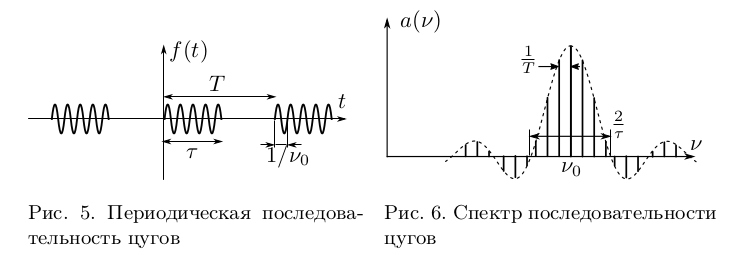
\includegraphics[width=.6\textwidth]{12.png}}

\noindent 13) При фиксированной длительности импульсов $\tau$ = 100 мкс исследуем зависимость расстояния $\delta\nu$ между соседними спектральными компонентами периода повторения импульсов T = 1/$nu_{\text{повт}}$ (в диапазоне частот 1-8 кГц)

\begin{center}
\begin{tabular}{|c|c|c|c|c|}
	\hline
	T, мкс & $\delta\nu_m$, кГц & $\delta\nu$, кГц & $\nu_{\text{повт}}$, кГц & m, шт \\
	\hline
	200 & 19,98 $\pm$ 0,02 & 4,995 $\pm$ 0,005 & 5,00 & 4 \\
	\hline
	300 & 19,98 $\pm$ 0,02 & 3,330 $\pm$ 0,003  & 3,33 & 6 \\
	\hline
	500 & 20,00 $\pm$ 0,02 & 2,000 $\pm$ 0,002 & 2,00 & 10 \\
	\hline
	800 & 12,52 $\pm$ 0,02 & 1,252 $\pm$ 0,002  & 1,25 & 10 \\
	\hline
	1100 & 9,10 $\pm$ 0,02 & 0,910 $\pm$ 0,002  & 0,91 & 10 \\
	\hline
	1500 & 6,66 $\pm$ 0,02  & 0,666 $\pm$ 0,002   & 0,67 & 10 \\
	\hline
	2000 & 5,06 $\pm$ 0,02  & 0,506 $\pm$ 0,002  & 0,50 & 10 \\
	\hline
	2500 & 4,00 $\pm$ 0,02  & 0,400 $\pm$ 0,002   & 0,40 & 10 \\
	\hline
	3000 & 3,34 $\pm$ 0,02  & 0,334 $\pm$ 0,002  & 0,33 & 10 \\
	\hline
	3500 & 2,86 $\pm$ 0,02  & 0,286 $\pm$ 0,002  & 0,29 & 10 \\
	\hline
	4000 & 2,50 $\pm$ 0,02  & 0,250 $\pm$ 0,002  & 0,25 & 10 \\
	\hline
	4500 & 2,22 $\pm$ 0,02  & 0,222 $\pm$ 0,002  & 0,22 & 10 \\
	\hline
	5000 & 2,00 $\pm$ 0,02  & 0,200 $\pm$ 0,002  & 0,20 & 10 \\
	\hline
\end{tabular}
\end{center}

\noindent 14) Построим график $\delta\nu$(1/T) и определим его наклон.

\end{document}
